% f1992nw_q26_cube_pyramid.tex — 1992 年·全国卷·文科 第 26 题（正方体与四棱锥）
%
% 【来源】`.work/phase4-b15/source/1992全国文.pdf`（SHA-256 8bd9671406dfcc344407488d75fa9eba95b62d02492aaeb728f8fd2fe193ffd6），
%   第 1 页（印刷页 43）；内容流逐路径实测见 `.work/phase4-b15/transcripts/arts-figures.md`。
%
% 【坐标口径】源 PDF 用户空间（原点左下、y 向上）。本图本地坐标
%   (x, y) = (x_page − 1027.0000, y_page − 251.0000)，1 单位 = 1 TeX pt。
%   路径坐标逐点照录内容流（含三次贝塞尔控制点）。
%
% 元素计数：14 条路径（7 实＋7 虚）＋10 个标签
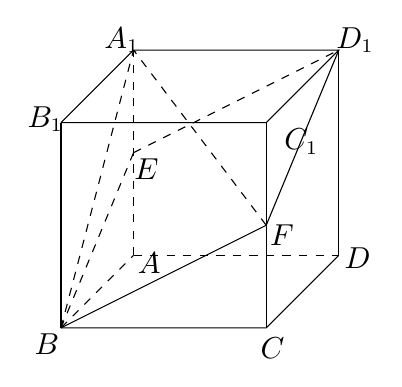
\begin{tikzpicture}[x=1pt, y=1pt,
    every node/.style={inner sep=0pt, font=\fontsize{10.5pt}{12.6pt}\selectfont}]
  \draw[line width=0.398pt] (5.6450,12.7860)   -- (79.8050,12.7860)   -- (106.0200,39.0010);
  \draw[line width=0.398pt] (5.6450,86.9458)   -- (79.8050,86.9458)   -- (106.0200,113.1608)   -- (31.8600,113.1608)   -- (5.6450,86.9458);
  \draw[line width=0.398pt] (79.8048,12.7860)   -- (79.8048,86.9460);
  \draw[line width=0.398pt] (106.0203,39.0015)   -- (106.0203,113.1615);
  \draw[line width=0.398pt] (5.6450,12.7860)   -- (5.6450,86.9460);
  \draw[line width=0.398pt] (79.8048,49.8659)   -- (5.6448,12.7859);
  \draw[line width=0.398pt] (79.8048,49.8659)   -- (106.0198,113.1609);
  \draw[line width=0.398pt, dash pattern=on 2.989pt off 2.989pt, dash phase=0.0pt] (5.6450,12.7860)   -- (31.8600,39.0010);
  \draw[line width=0.398pt, dash pattern=on 2.989pt off 2.989pt, dash phase=0.0pt] (31.8605,39.0015)   -- (106.0205,39.0015);
  \draw[line width=0.398pt, dash pattern=on 2.989pt off 2.989pt, dash phase=0.0pt] (31.8605,39.0015)   -- (31.8605,113.1615);
  \draw[line width=0.398pt, dash pattern=on 2.989pt off 2.989pt, dash phase=0.0pt] (31.8605,76.0814)   -- (5.6455,12.7864);
  \draw[line width=0.398pt, dash pattern=on 2.989pt off 2.989pt, dash phase=0.0pt] (31.8605,76.0814)   -- (106.0205,113.1614);
  \draw[line width=0.398pt, dash pattern=on 2.989pt off 2.989pt, dash phase=0.0pt] (79.8048,49.8659)   -- (31.8608,113.1609);
  \draw[line width=0.398pt, dash pattern=on 2.989pt off 2.989pt, dash phase=0.0pt] (5.6450,12.7860)   -- (31.8600,113.1610);

  \node[anchor=center] at (111.900,116.700) {$D_1$};  % 源中心 (1138.90,367.70)
  \node[anchor=center] at (0.000,88.200) {$B_1$};  % 源中心 (1027.00,339.20)
  \node[anchor=center] at (92.500,80.000) {$C_1$};  % 源中心 (1119.50,331.00)
  \node[anchor=center] at (27.700,116.700) {$A_1$};  % 源中心 (1054.70,367.70)
  \node[anchor=center] at (112.800,38.000) {$D$};  % 源中心 (1139.80,289.00)
  \node[anchor=center] at (82.100,5.400) {$C$};  % 源中心 (1109.10,256.40)
  \node[anchor=center] at (0.500,6.900) {$B$};  % 源中心 (1027.50,257.90)
  \node[anchor=center] at (37.500,36.000) {$A$};  % 源中心 (1064.50,287.00)
  \node[anchor=center] at (36.500,70.200) {$E$};  % 源中心 (1063.50,321.20)
  \node[anchor=center] at (85.500,46.200) {$F$};  % 源中心 (1112.50,297.20)

\end{tikzpicture}
%
% 【自验结果】
%   探针：见 .work/phase4-b15/probe 的 verify_paths.py / check600_b15.py。
